We inspect two existing parity game algorithms which will be used in VPG algorithms. First Zielonka's recursive algorithm which is well studied and generally considered to be the best performing parity game algorithm. We also inspect the fixed-point iteration algorithm which tends to perform well for model-checking problems with a low number of distinct priorities.

\subsection{Zielonka's recursive algorithm}
First we consider Zielonka's recursive algorithm, created from the constructive proof given in \cite{ZIELONKA1998135}, which solves total PGs. Pseudo code is presented in algorithm \ref{alg_zlnk_org}.
\begin{algorithm}
	\caption{$\textsc{RecursivePG}(\textit{PG } G = (V,V_0,V_1, E, \Omega))$}
	\label{alg_zlnk_org}
	\begin{algorithmic}[1]
		\State $m \gets \min\{ \Omega(v)\ |\ v \in V\}$
		\State $h \gets\max\{ \Omega(v)\ |\ v \in V\}$
		\If{$h = m$ or $V = \emptyset$}
		\If{$h$ is even or $V = \emptyset$}
		\State \Return $(V,\emptyset)$
		\Else
		\State \Return $(\emptyset, V)$
		\EndIf
		\EndIf
		\State $\alpha \gets 0$ if $h$ is even and $1$ otherwise
		\State $U \gets \{v \in V\ |\ \Omega(v) = h\}$
		\State $A \gets \alpha\textit{-Attr}(G, U)$
		\State $(W_0', W_1') \gets \textsc{RecursivePG}(G \backslash A)$
		\If{$W_{\overline{\alpha}}' =\emptyset$}
		\State $W_\alpha \gets A \cup W_\alpha'$
		\State $W_{\overline{\alpha}} \gets \emptyset$
		\Else
		\State $B \gets \overline{\alpha}\textit{-Attr}(G,W_{\overline{\alpha}}')$
		\State $(W_0'', W_1'') \gets \textsc{RecursivePG}(G \backslash B)$
		\State $W_\alpha \gets W_\alpha''$
		\State $W_{\overline{\alpha}} \gets W_{\overline{\alpha}}'' \cup B$
		\EndIf
		\State \Return $(W_0, W_1)$
	\end{algorithmic}
\end{algorithm}

The algorithm works for solving $G$ by taking the set of vertices with the highest priority and choosing player $\alpha$ such that $\alpha$ has the same parity as the highest priority. Next the algorithm finds all the vertices such that player $\alpha$ can force the play to one of these high priority vertices. Next this set of vertices is removed from the game and the resulting subgame is solved recursively. This subgame returns winning sets $W'_0$ and $W'_1$. Vertices in set $W'_{\overline{\alpha}}$ are won by player $\overline{\alpha}$ in the subgame but are also won by player $\overline{\alpha}$ in $G$. The algorithm tries to find all the vertices in $G$ such that player $\overline{\alpha}$ can force the play to a vertex in $W'_{\overline{\alpha}}$ and therefore winning the game. We now have a set of vertices that are definitely won by player $\overline{\alpha}$ in game $G$. In the rest of the game player $\alpha$ can keep the play from $W'_{\overline{\alpha}}$ so the algorithm solves the rest of the game recursively to find the complete winning sets for game $G$.

 A complete explanation of the algorithm can be found in \cite{ZIELONKA1998135}, we do introduce definitions for the attractor set and for subgames. 
 
 An attractor set is a set of vertices $A \subseteq V$ calculated for player $\alpha$ given set $U \subseteq V$ where player $\alpha$ has a strategy to force the play starting in any vertex in $A \backslash U$ to a vertex in $U$.


\begin{definition}\cite{ZIELONKA1998135}
	\label{def_attr}Given parity game $G = (V,V_0,V_1,E,\Omega)$ and a non-empty set $U \subseteq V$ we define $\alpha\textit{-Attr}(G,U)$ such that
	\[U_0 = U \]
	For $i \geq 0$:
	\begin{align*}
	U_{i+1} = U_i\cup
	&\{v \in V_\alpha\ |\ \exists v' \in V : v' \in U_i \wedge (v,v') \in E \}\\
	\cup &\{v \in V_{\overline{\alpha}}\ |\ \forall v' \in V :(v,v') \in E \implies v' \in U_i \}
	\end{align*}
	Finally:
	\[\alpha\textit{-Attr}(G,U) = \bigcup_{i \geq 0} U_i \]
\end{definition}

The algorithm creates subgames, where a set of vertices is removed from a parity game to create a new parity game.

\begin{definition}\cite{ZIELONKA1998135}
	\label{def_org_subgame}
	Given a parity game $G = (V,V_0,V_1, E,\Omega)$ and $U \subseteq V$ we define the subgame $G \backslash U$ to be the game $(V', V_0', V_1', E', \Omega)$ with:
	\begin{itemize}
		\item $V' = V \backslash U$,
		\item $V_0' = V_0 \cap V'$,
		\item $V_1' = V_1 \cap V'$ and
		\item $E' = E \cap (V' \times V')$.
	\end{itemize}
\end{definition}

Note that a subgame is not necessarily total, however the recursive algorithm always creates subgames that are total (shown in \cite{ZIELONKA1998135}).

\subsubsection{Zielonka's recursive algorithm local}
\label{sec:zlnk_org_local}
We can modify Zielonka's algorithm to solve parity games locally. We use the property that vertices won by player $\overline{\alpha}$ in game $G \backslash A$ are also won by player $\overline{\alpha}$ in game $G$. We use this property to, in some cases, not go into the second recursion because we already found the vertex. We extend the algorithm with two parameters, $v_0$ and $\Delta$. Vertex $v_0$ represents the vertex that we try to solve. Parameter $\Delta \subseteq \{0,1\}$ contains a set of players for which we try to find vertex $v_0$, if we find $v_0$ to be won by a player that is in $\Delta$ we are done for that recursion. However if we find vertex $v_0$ to be won by a player that is not in $\Delta$ we need to solve the entire game. The algorithm can make use of this to tell a recursive call it needs to find the vertex to be won by player $\overline{\alpha}$ in the subgame because then this vertex is also won by player $\overline{\alpha}$ in the game itself. If the vertex is not won by $\overline{\alpha}$ the entire game needs to be solved because the winning sets are required in the second recursion. Pseudo code for the algorithm is provided in algorithm \ref{alg_zlnk_local}.
\begin{algorithm}
	\caption{$\textsc{RecursivePGLocal}(\textit{PG } G = (V,V_0,V_1, E, \Omega),v_0,\Delta)$}
	\label{alg_zlnk_local}
	\begin{algorithmic}[1]
		\State $m \gets \min\{ \Omega(v)\ |\ v \in V\}$
		\State $h \gets\max\{ \Omega(v)\ |\ v \in V\}$
		\If{$h = m$ or $V = \emptyset$}
		\If{$h$ is even or $V = \emptyset$}
		\State \Return $(V,\emptyset)$
		\Else
		\State \Return $(\emptyset, V)$
		\EndIf
		\EndIf
		\State $\alpha \gets 0$ if $h$ is even and $1$ otherwise
		\State $U \gets \{v \in V\ |\ \Omega(v) = h\}$
		\State $A \gets \alpha\textit{-Attr}(G, U)$
		\If{$\overline{\alpha} \in \Delta$}
		\State $(W_0', W_1') \gets \textsc{RecursivePGLocal}(G \backslash A,v_0,\{\overline{\alpha}\})$
		\Else
		\State $(W_0', W_1') \gets \textsc{RecursivePGLocal}(G \backslash A,v_0,\emptyset)$
		\EndIf
		\If{$W_{\overline{\alpha}}' =\emptyset$}
		\State $W_\alpha \gets A \cup W_\alpha'$
		\State $W_{\overline{\alpha}} \gets \emptyset$
		\Else
		\If{$\overline{\alpha} \in \Delta \wedge v_0 \in W'_{\overline{\alpha}}$}
		\State $(W_0,W_1) \gets (W'_0, W'_1)$
		\Else
		\State $B \gets \overline{\alpha}\textit{-Attr}(G,W_{\overline{\alpha}}')$
		\If{$\overline{\alpha} \in \Delta \wedge v_0 \in B$}
		\State $W_\alpha \gets \emptyset$
		\State $W_{\overline{\alpha}} \gets B$
		\Else
		\State $(W_0'', W_1'') \gets \textsc{RecursivePGLocal}(G \backslash B,v_0,\Delta)$
		\State $W_\alpha \gets W_\alpha''$
		\State $W_{\overline{\alpha}} \gets W_{\overline{\alpha}}'' \cup B$
		\EndIf
		\EndIf
		\EndIf
		\State \Return $(W_0, W_1)$
	\end{algorithmic}
\end{algorithm}
\begin{theorem}
	Given total parity game $G = (V,V_0,V_1,E,\Omega)$, vertex $v_0$ (which is not necessarily in $V$), $\Delta \subseteq \{0,1\}$ and winning sets $Q_0$ and $Q_1$ for game $G$. We have for sets $(W_0,W_1) = \textsc{RecursivePGLocal}(G,v_0,\Delta)$ that either or both of the following statements hold:
	\begin{enumerate}[(I)]
		\item For some $\beta \in \{0,1\}$ we have $v_0 \in W_\beta$, $v_0 \in Q_\beta$ and $\beta \in \Delta$.
		\item $W_0 = Q_0$ and $W_1 = Q_1$.
	\end{enumerate}
\begin{proof}
	To prove the correctness we compare the behaviour of \textsc{RecursivePGLocal} with the behaviour of the original algorithm \textsc{RecursivePG} for which we know that it is correct.
	
	Prove by induction on $G$:
	
	\textbf{Base: } When there are no vertices in $V$ or there is only one priority then the local algorithm behaves the same as the original algorithm so statement (II) holds.
	
	
	\textbf{Step: } We start by distinguishing two cases, first we assume that $v_0 \notin V$. Vertex $v_0$ is also not in any subgame of $G$. In the first recursion we know by induction that either or both of the statements are true for $G\backslash A$, since $v_0$ is not in game $G\backslash A$ only statement (II) can be true. So the first recursion returns the same result as the original algorithm would. The if statements guarding the second recursion are always false because $v_0 \notin B$ and $v_0 \notin W'_{\overline{\alpha}}$ and similarly as with game $G\backslash A$ the vertex $v_0$ is not in $G\backslash B$. So the second recursion also returns the same values as the original algorithm would. We can conclude that when $v_0 \notin V$ the local algorithm behaves the same as the original and therefore statement (II) holds.
	
	Now consider $v_0 \in V$. Again we distinguish two cases, starting with $\overline{\alpha} \notin \Delta$. In the first recursive call we get $\Delta = \emptyset$, by induction either or both statements hold for $G\backslash A$, however with $\Delta = \emptyset$ statement (II) must be true. Therefore the first recursive call behaves the same as the original algorithm. The if statements guarding the second recursion are always false since $\overline{\alpha} \notin \Delta$ so the second recursive call is always performed. Up until this second recursive call the local algorithm behaves the same as the original algorithm. From the correctness of the original algorithm we can conclude that vertices won by some player in game $G\backslash B$ are also won by that player in game $G$. This holds true in the local algorithm since it has behaved identical up to this point. By induction we know either or both statements are true, if statement (II) is true for $G\backslash B$ then the algorithm behaves the same as the original and statement (II) is also true for game $G$. If statement (I) is true for $G \backslash B$ and $v_0$ is won by player $\beta$ in $G\backslash B$ then we know $v_0$ is also won by player $\beta$ in game $G$ and thus statement (I) holds for $G$.
	
	Next consider $\overline{\alpha} \in \Delta$ (and $v_0 \in V$). The first recursive call is made with $\Delta = \{\overline{\alpha}\}$. If $W'_{\overline{\alpha}} = \emptyset$ then statement (II) must be true for game $G\backslash A$ and the algorithm behaves the same as the original in which case statement (II) is true for $G$. If $W'_{\overline{\alpha}} \neq \emptyset$ then we consider $v_0$ being in $W'_{\overline{\alpha}}$, by induction we can conclude that $v_0$ is indeed won by player $\overline{\alpha}$ in game $G\backslash A$. Furthermore from the correctness of the original algorithm we can conclude that any vertex won by player $\overline{\alpha}$ in game $G\backslash A$ is also won by player $\overline{\alpha}$ in game $G$. So returning winning sets $W'_0$ and $W'_1$ make statement (I) true for game $G$.
	
	Consider $v_0$ not being in $W'_{\overline{\alpha}}$ but in $B$. We can conclude that statement (II) is true for subgame $G\backslash A$ so the algorithm behaves the same as the original algorithm up until this point. Using the original algorithm we can see that any vertex in $B$ is won by player $\overline{\alpha}$ in game $G$ so if we find $v_0$ in $B$ we can return $B$ for player $\overline{\alpha}$ which includes $v_0$ and $\emptyset$ for player $\alpha$ to make statement (I) true for game $G$.
	
	If $v_0$ is also not in $B$ then we still conclude that statement (II) is true for subgame $G\backslash A$ and that the algorithm has behaved the same as the original algorithm up until this point. From the correctness of the original algorithm we can conclude that vertices won by some player in game $G\backslash B$ are also won by that player in game $G$. This holds true in the local algorithm since it has behaved identical up to this point. By induction we know either or both statements are true, if statement (II) is true for $G\backslash B$ then the algorithm behaves the same as the original and statement (II) is also true for game $G$. If statement (I) is true for $G \backslash B$ and $v_0$ is won by player $\beta$ in $G\backslash B$ then we know $v_0$ is also won by player $\beta$ in game $G$ and thus statement (I) holds for $G$.
\end{proof}
\end{theorem}

Calling $\textsc{RecursivePGLocal}(G, v_0, \{0,1\})$ with $v_0$ in $G$ either solves the full game (statement (II)) or correctly puts $v_0$ in either winning set (statement (I)). In both cases $v_0$ is in the correct winning set and the game is solved locally.

The algorithm uses the property that vertices won by player $\overline{\alpha}$ in a subgame during the algorithm are also won by player $\overline{\alpha}$ in the game itself. However this property only goes one recursion deep, meaning that during the solving of a game there can be a subsubgame where a vertex is won by player $\overline{\alpha}$ however in the original game we try to solve this vertex is won by player $\alpha$. For this reason the local algorithm can't simply claim to be done when $v_0$ is won by $\overline{\alpha}$, but we need to pass down a value for $\Delta$.

We disprove the following conjecture to show that there indeed can be a vertex that is won by player $\overline{\alpha}$ at some point but be won by player $\alpha$ in a higher recursion level.
\begin{conjecture}[Disproven]
	For any $\textsc{RecursivePG}(G')$ that is invoked during $\textsc{RecursivePG}(G)$ it holds that any vertex $v \in W'_{\overline{\alpha}}$ is won by player $\overline{\alpha}$ in game $G$.
\end{conjecture}
We disprove this conjecture using the following counter example $G$:\\
\begin{center}
	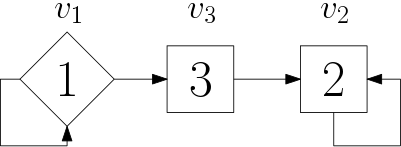
\includegraphics[scale=0.5]{counterexampleBconjecture}\\
\end{center}
All vertices are won by player $0$ ($v_1$ plays to $v_3$, $v_3$ must play to $v_2$ and $v_2$ must play to itself therefore we always get an infinite path of $v_2$'s).\\
We solve this game using \textsc{RecursivePG} and write down the values of relevant variables below. We use the hat decoration to indicate values for variables in the first recursion:\\
\begin{tabular}{|p{20cm}}
$\textsc{RecursivePG}(G)$:\\
$h=3$,$\alpha=1$\\
$A =\{v_3\}$\\
\begin{tabular}{|p{20cm}}
	$\textsc{RecursivePG}(G\backslash A)$:\\
	$\hat{h}=2,\hat{\alpha}=0$\\
	$\hat{A}=\{v_2\}$\\
	\begin{tabular}{|p{20cm}}
		$\textsc{RecursivePG}(G\backslash A\backslash \hat{A})$\\
	\end{tabular}
	$\hat{W}'_0 = \emptyset$\\
	$\hat{W}'_1 = \{v_1\} = \hat{W}'_{\overline{\hat{\alpha}}}$\\
	\textbf{Vertex $v_1$ is in $\hat{W}'_{\overline{\hat{\alpha}}}$ however in $G$ the vertex is won by player} $\hat{\alpha}$.\\
	$\hat{B} = \{v_1\}$\\
	\begin{tabular}{|p{20cm}}
		$\textsc{RecursivePG}(G\backslash A\backslash \hat{B})$\\
	\end{tabular}
	$\hat{W}''_0 = \{v_2\}, \hat{W}''_1 = \emptyset$\\
\end{tabular}
$W'_0 = W'_{\overline{\alpha}} = \{v_2\}$\\
$W'_1 = W'_\alpha = \{v_1\}$\\
$B = V$\\
$W_0 = V$
\end{tabular}
\subsection{Fixed-point iteration algorithm}
Parity games can be solved by solving an alternating fixed-point formula, as shown in \cite{WALUKIEWICZ2002311}. We will consider PG $G = (V,V_0,V_1, E, \Omega)$ with $d$ distinct priorities. We can apply \textit{priority compression} to make sure every priority in $G$ maps to a value in $\{0,\dots,d-1\}$ or $\{1, \dots, d\}$ \cite{SolvingInPractice,FPITE}. We assume without loss of generality that the priorities map to $\{0,\dots,d-1\}$ and that $d-1$ is even. 

Consider the following formula
\[ S(G = (V,V_0,V_1,E,\Omega)) = \nu Z_{d-1}. \mu Z_{d-2}. \dots . \nu Z_0. F_0(Z_{d-1},\dots,Z_0) \]
with
\[ F_0(Z_{d-1},\dots,Z_0) = \{ v \in V_0\ |\ \exists_{w\in V} (v,w) \in E \wedge Z_{\Omega(w)} \} \cup \{ v \in V_1\ |\ \forall_{w\in V} (v,w) \in E \implies Z_{\Omega(w)} \} \]
where $Z_i \subseteq V$. The formula $\nu X. f(X)$ solves the greatest fixed-point of $X$ in $f$, similarly $\mu X.f(X)$ solves the least fixed-point of $X$ in $f$.

To understand the formula we consider sub-formula $\nu Z_0. F_0(Z_{d-1},\dots,Z_0)$. This formula holds for vertices from which player $0$ can either force the play into a node with priority $i > 0$ for which $Z_i$ holds or the player can stay in vertices with priority $0$ indefinitely. The formula $\mu Z_0. F_0(Z_{d-1},\dots,Z_0)$ holds for vertices from which player $0$ can force the play into a node with priority $i > 0$ for which $Z_i$ holds in finitely many steps. For an extensive treatment we refer to \cite{WALUKIEWICZ2002311}.

We further inspect formula $S$. Given game $G$, consider the following subformula's:
\[ S^{d-1}(Z_{d-1}) = \mu Z_{d-2}.S^{d-2}(Z_{d-2})\]
\[ S^{d-2}(Z_{d-2}) = \nu Z_{d-3}.S^{d-3}(Z_{d-3})\]
\begin{center}
	\dots
\end{center}
\[ S^{0}(Z_0) = F_0(Z_{d-1},\dots,Z_0)\]
The fixed-point variables are all elements of $2^V$, therefore we have for every subformula the following type:
\[ S^i(Z_i) : 2^V \rightarrow 2^V \]
Furthermore, since $V$ is finite, the partially ordered set $\langle 2^V, \subseteq \rangle$ is a complete lattice.

Finally every subformula is $S^i(Z_i)$ is monotonic, ie. if $S^i(Z_i) \geq S^i(Z_i')$ then $Z_i \geq Z_i'$.

\subsubsection{Fixed-point iteration}
Fixed-point formula's can be solved by fixed-point iteration. As shown in \cite{Emerson:1986:MCP:900378} we can calculate $\mu X.f(X)$, where $f$ is monotonic in $X$ and $X \in 2^V$, by iterating $X$:
\[ \mu X.f(X) = \bigcup_{i \geq 0} X^i \]
where $X^i = f(X^{i-1})$ for $i > 0$ and $X^0 \subseteq \mu X.f(X)$. So picking the smallest value possible for $X_0$ will always correctly calculate $\mu X. f(X)$.

Similarly we can calculate fixed-point $\nu X.f(X)$ when $f$ is monotonic in $X$ by iterating $X$.
\[ \nu X.f(X) = \bigcap_{i \geq 0} X^i \]
where $X^i = f(X^{i-1})$ for $i > 0$ and $X^0 \supseteq \nu X.f(X)$. So picking the largest value possible for $X_0$ will always correctly calculate $\nu X. f(X)$.

Since every subformula is monotonic and maps from a value in $2^V$ to another value in $2^V$ we can apply fixed-point iteration to solve the subformula's, we choose initial values $\emptyset$ for least fixed-point variables and $V$ for greatest fixed-point variables.

An algorithm to perform the iteration is presented in \cite{FPITE} and shown in algorithm \ref{alg_FPITEorg}.
\begin{algorithm}
	\caption{Fixed-point iteration}
	\label{alg_FPITEorg}
	\begin{multicols}{2}
		\begin{algorithmic}[1]
			\Function{FPIter}{$G = (V, V_0, V_1, E, \Omega)$}
			\For{$i \gets d-1,\dots,0$}
			\State $\textsc{Init}(i)$
			\EndFor
			\Repeat
			\State $Z_0'\gets Z_0$
			\State $Z_0 \gets \textsc{Diamond}() \cup \textsc{Box}()$
			\State $i \gets 0$
			\While{$Z_i=Z_i' \wedge i < d-1$}
			\State $i \gets i+1$
			\State $Z_i' \gets Z_i$
			\State $Z_i \gets Z_{i-1}$
			\State $\textsc{Init}(i-1)$
			\EndWhile
			\Until{$i = d-1 \wedge Z_{d-1} = Z_{d-1}'$}
			\State \Return $(Z_{d-1},V\backslash Z_{d-1})$
			\EndFunction
		\end{algorithmic}\bigskip\bigskip
		\begin{algorithmic}[1]
			\Function{Init}{$i$}
			\State $Z_i \gets \emptyset$ if $i$ is odd, $V$ otherwise
			\EndFunction
		\end{algorithmic}\bigskip
		\begin{algorithmic}[1]
			\Function{Diamond}{}
			\State \Return $\{ v \in V_0\ |\ \exists_{w\in V} (v,w) \in E \wedge w \in Z_{\Omega(w)}\}$
			\EndFunction
		\end{algorithmic}\bigskip
		\begin{algorithmic}[1]
			\Function{Box}{}
			\State \Return $\{ v \in V_1\ |\ \forall_{w\in V} (v,w) \in E \implies w \in Z_{\Omega(w)}\}$
			\EndFunction
		\end{algorithmic}
	\end{multicols}
\end{algorithm}

\subsubsection{Fixed-point iteration local}
We can modify the fixed-point iteration algorithm to solve a game locally by distinguishing two cases:
\begin{enumerate}
	\item If $d-1$ is even then the outermost fixed-point variable is a greatest fixed-point variable. When at some point $v_0 \notin Z_{d-1}$ then we know $0$ is never won by player $1$ and we are done.
	\item If $d-1$ is odd then the outermost fixed-point variable is a least fixed-point variable. When at some point $v_0 \in Z_{d-1}$ then we know $0$ is won by player $0$ and we are done.
\end{enumerate}